\documentclass[paper=letter, fontsize=11pt]{scrartcl} % A4 paper and 11pt font size
\synctex=1
\usepackage[T1]{fontenc} % Use 8-bit encoding that has 256 glyphs
\usepackage{fourier} % Use the Adobe Utopia font for the document - comment this line to return to the LaTeX default
\usepackage[english]{babel} % English language/hyphenation
\usepackage{amsmath,amsfonts,amsthm} % Math packages
%\usepackage[nolists, nomarkers]{endfloat}
\usepackage{hyperref}
\usepackage{bm}
\usepackage{graphicx}
\usepackage[section]{placeins}
\usepackage{sectsty} % Allows customizing section commands
\allsectionsfont{\normalfont\scshape} % Make all sections centered, the default font and small caps

\usepackage{fancyhdr} % Custom headers and footers
\pagestyle{fancyplain} % Makes all pages in the document conform to the custom headers and footers
\fancyhead{} % No page header - if you want one, create it in the same way as the footers below
\fancyfoot[L]{} % Empty left footer
\fancyfoot[C]{} % Empty center footer
\fancyfoot[R]{\thepage} % Page numbering for right footer
\renewcommand{\headrulewidth}{0pt} % Remove header underlines
\renewcommand{\footrulewidth}{0pt} % Remove footer underlines
\setlength{\headheight}{13.6pt} % Customize the height of the header

\numberwithin{equation}{section} % Number equations within sections (i.e. 1.1, 1.2, 2.1, 2.2 instead of 1, 2, 3, 4)
\numberwithin{figure}{section} % Number figures within sections (i.e. 1.1, 1.2, 2.1, 2.2 instead of 1, 2, 3, 4)
\numberwithin{table}{section} % Number tables within sections (i.e. 1.1, 1.2, 2.1, 2.2 instead of 1, 2, 3, 4)

\setlength\parindent{0pt} % Removes all indentation from paragraphs -
                          % comment this line for an assignment with
                          % lots of text
\setlength\parskip{12pt}


%----------------------------------------------------------------------------------------
%   TITLE SECTION
%----------------------------------------------------------------------------------------

\newcommand{\horrule}[1]{\rule{\linewidth}{#1}} % Create horizontal rule command with 1 argument of height

\title{ 
\normalfont \normalsize 
\textsc{Exoplanet Patchy Cloud Project} \\ [25pt] % Your university, school and/or department name(s)
\horrule{0.5pt} \\[0.4cm] % Thin top horizontal rule
\huge Reply to Daniel \& Glenn\\ % The assignment title
\horrule{2pt} \\[0.5cm] % Thick bottom horizontal rule
}

\author{Yifan Zhou}
\date{\normalsize\today} % Today's date or a custom date

\usepackage{scalerel}
\usepackage{calc}
\global\newcounter{embedlevel}
\global\newlength\embedspace
\embedspace=2ex
\setcounter{embedlevel}{1}
\newcommand\embed[1]{%
  \stepcounter{embedlevel}%
  \stretchrel{\rule{0.2ex}{1ex}}{\hspace{1.8ex}\parbox{%
    \textwidth-\value{embedlevel}\embedspace}{%
    \rule{0ex}{2ex}\textbf{\textit{#1}}\rule[-1.3ex]{0ex}{1.3ex}%
  }}%
  \vspace{.5ex}%
  \addtocounter{embedlevel}{-1}%
}
\begin{document}

\maketitle % Print the title
\section{Clarifications}
\embed{
1) How do you scale (if you scale) the residuals you subtract?
}

The residuals are not scaled. I simply took the median of the
residuals that have the same dither position and position angle, and
subtracted the median combination from the original images. Since The
chisq distribution of the fitting looks very reasonable for me, I did
not attempt to make further adjustment of the residual models.

\embed{
 2) How do the residuals images look like? What is the relative
 fraction of the light that is not subtracted well?
}

\embed{
 3) When you calculate the brightness of the sources, how do you use
 the information of the residuals and the TinyTim-based PSF?
}

These are very important points. However I did not deal with them very
carefully in the fit. As I showed in our previous discussion,
Tinytim does not provide a precise PSF model so that the residual of
tinytim PSF subtraction has a 2\% - 4\% average relative fraction of
original image(mean(residual/image) $\sim$ 2\%-\%4). For the fitting routine I used this
time,  the fluxes of A and B purely calculated from the
amplitudes of the two components of the PSF. I did not count any flux
from the residual model into the fluxes of A or B.

An average relative fraction of 2-4\% of the residual model could be a
significant source of uncertainty. Especially for the case that I
ignored the flux from the residual totally. However, I have not come up
with any ideas on including the residual flux to the final result. I
think we need further discussion about this point.

\embed{ a) When you say you carried out a "two component tinytim PSF
  fit", it is not clear to me what you mean.  I assume the linear
  superposition of two TinyTim PSFs.  But do you mean one for A and
  one for B that are otherwise identical (or perhaps different in some
  manner other than brightness?).  Or do you mean for B (and perhaps
  also A) you have used a combination of TinyTim PSFs that, in
  combination (perhaps with different defocus of color terms?) better
  represent the observed PSF?  }

I used different PSFs for A and B. My fitting routine firstly
generates a list of PSFs using the position of A and the NIR spectrum
of A (Bonnefoy et. al. 2014) with different telescope jittering. I fit
this PSF to the image of A with an area where the image of B is mostly
excluded ( using a 3-pixel radius mask centered on B) to find the best
matched position and Jittering. Next, I used this jittering to
generate a PSF of B with B's position on detector and B's spectrum
(Patience et al. 2010). In the third step, I fit the two PSFs together
with the position of A fixed , and to find the best matched position
of B and amplitudes of 2 PSFs.

\embed{
b) To me it is interesting (but not really unexpected) that binning
by "same position angle" (i.e., spacecraft roll angle) improves.
Off-rolling does thermally destablise the PSF to some extent - by
changing the angle to the sub-solar point on the Earth as the
telescope orbits and can drive quasi-breathing modes.  I am a bit
surprised that these stabilize out as well as they seem to do (as
exhibited by the factor of 10 improvement in chisq).  It would be
interesting to know how much of that improvement is do to "same
dither position" and how much to "same roll" (as differently binned).
I am sure they both play together to reduce the residuals, but
knowing this could have influence on how future observations might be
constructed.}


The position dependency of the residual pattern comes from at least
three parts.
\begin{enumerate}
\item  Instrumental as Glenn described 
\item The imperfection of flat
  field is not modeled with TinyTim. 
\item  The PSFs are sampled
  differently at different position with a low sample rate.
\end{enumerate}


It is actually difficult to differentiate the improvement in terms of
different instrumental effect, since the there are significant
uncertainty and artifect generated by last two points.

\embed{
Overall, these look good; the question is, of course, how much of the
apparent trend is real.  One note here: It is curious how both A and B
have an increase in the first 3 orbits and then a different behavior
in orbits 4-6.}

\embed{
Could you explain how exactly do you determine the normalization
factors for the different angles/dithering positions?}

I median combined the fluxes calculated with images taking with same
filter, dithering position and roll angles, and devided the median
combination from every photometric result of these exposures.

\section{Discussion and further analysis}
\embed{
Daniel asks: "how much of the apparent trend is real".  This might be
difficult to ascertain.  Clearly the F125W and F160W for A seem well
correlated (1st 3 vs last 3 orbits) , but that correlation possibly
could still be instrumental.  If you took the new light curves as
binned, for B:
}

\embed{
if you average all the points together in each orbit (loosing the
 finer temporal information) is the change in normalized flux for B
 over the six orbits also "consistent" from F125W to F160W **AND** is it
 correlated with A?  It's a little harder to tell (quantitatively) as
 plotted for B simply because it is noisier than A.  In both A and B
 (both bands) the flux (by eye) also seems lower in the last three
 orbits and MAYBE the is a small secular rise in orbits 1-3.  I would
 expect that behavior in A and B to be independent, whereas if
 correalted that may be an instrumental signature.}

I binned the light curve of A and B by orbits using average. According to the result
I obtained, there are no clear correlation/anti-correlation betwee the
fluxes of A and B. Figure \ref{fig:1} presented the orbit-binned light
curves.

\begin{figure}
  \centering
  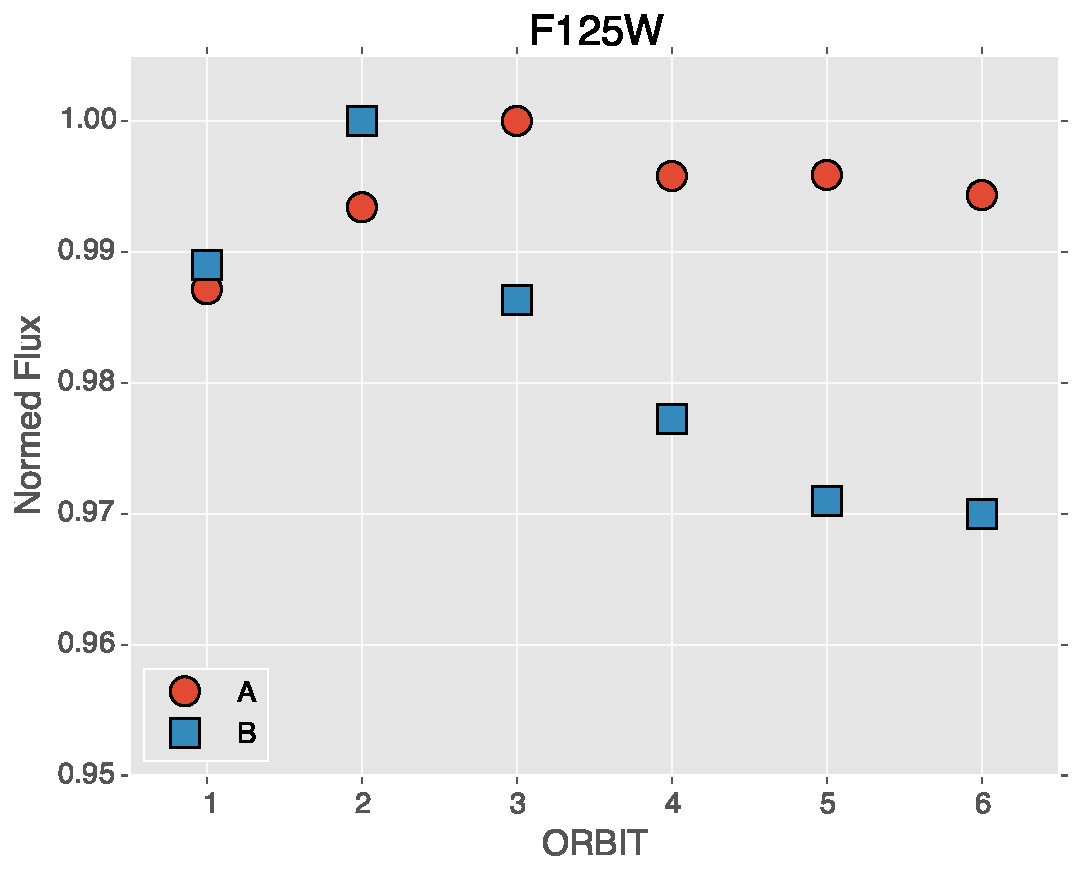
\includegraphics[width=0.45\textwidth]{binned_coor_F125W}
  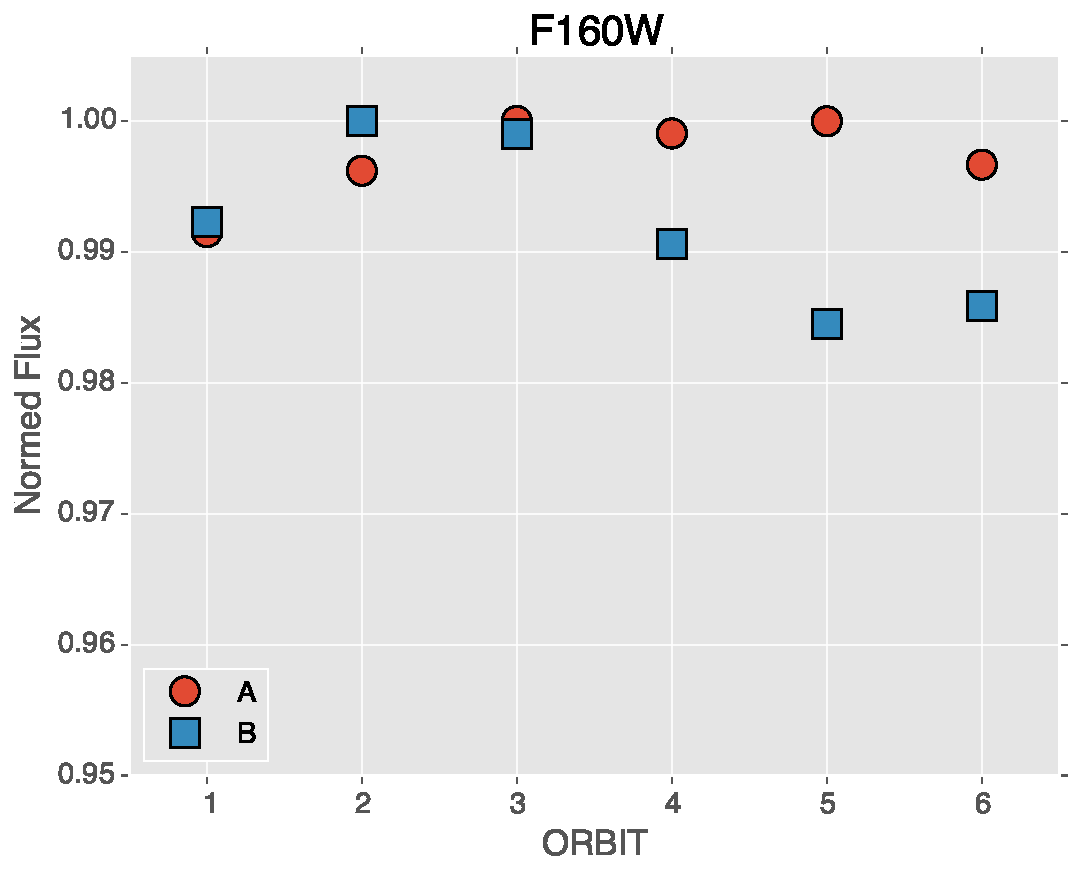
\includegraphics[width=0.45\textwidth]{binned_coor_F160W}
  \caption{Orbit-binned light curves. Binned curve for B showed a sine
  wave shaped curve}
  \label{fig:1}
\end{figure}

\embed{
This looks quite nice and indeed, the 10.9 hours is not a period that
I would obviously associate with an instrumental artifact.  Have you
tried the same for the F160W LC? It would be a nice verification if
you would get a similar periodicity.}

By eye, unbinned light curve of F160W does not show a sine-wave like
shape. However, in the orbit-binned curve, the light curve of B showed
a sine wave shaped curve as shown in Figure \ref{fig:1}. For F160W LC
of B, The least square fit results in a sine curve with a period of
9.3 hr. I also tried to fit the F160W light curve with a sine curve
that has a fixed period of 10.9 hr. I plotted the two best fit sine
curves together with the original observation points as in Figure
\ref{fig:2}. Considering the large scattering of photometric
measurement of B, it is actually hard to tell from Figure \ref{fig:2} whether
the 9.3 hr light curve fits better than the 10.9 hr light curve.

\begin{figure}[h!]
  \centering
  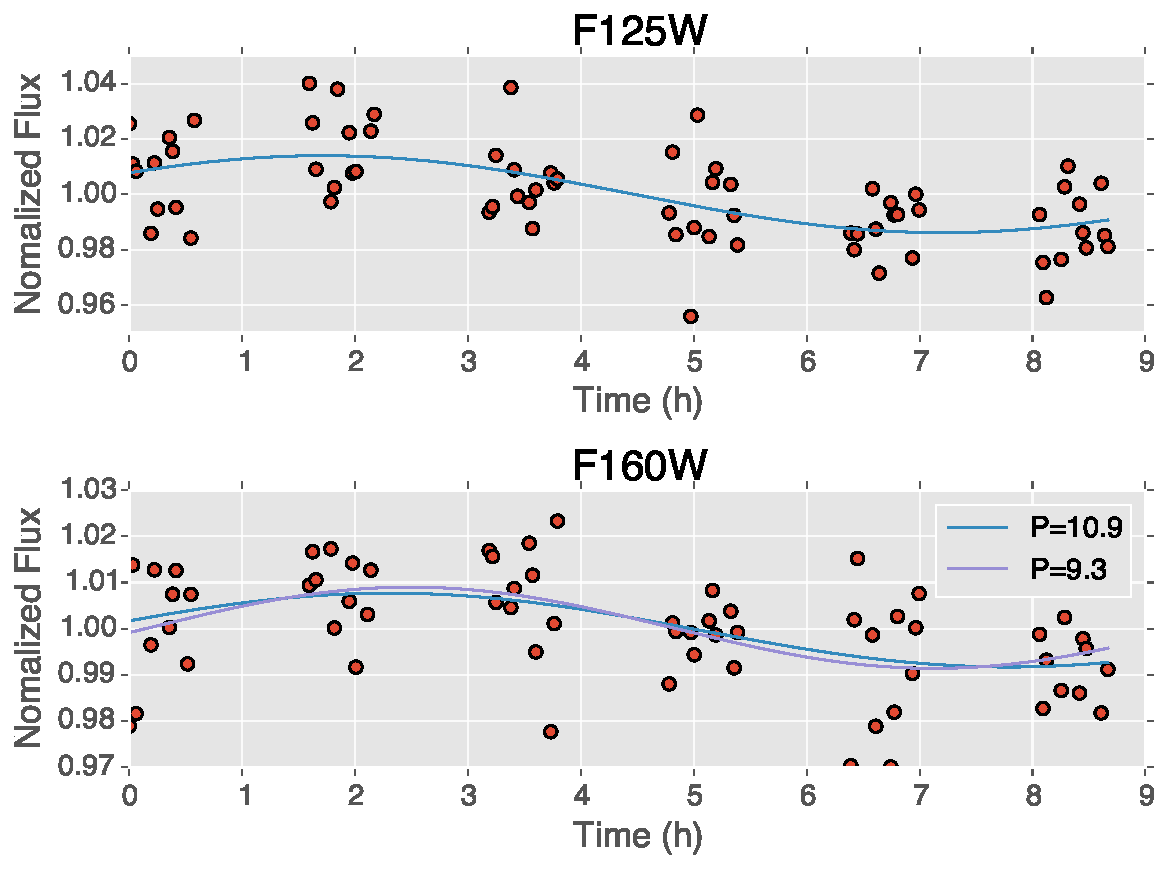
\includegraphics[width=0.8\textwidth]{sineCurveFit}
  \caption{sinusoidal wave fit to the light curve of 2M1207B. For the
    F160W panel, two curves for periods of 9.3 hr and 10.9 hr are
    plotted.}
  \label{fig:2}
\end{figure}

\embed{
Also, to be consistent, can you please use the same fitting procedure
for A (in both filters) and send similar plots?}

I did the fitting for A in both fittings. The rise in first three
orbits is the main feature that defines the sinusoidal wave. However
if it were truly part of a sin wave, the sine function would not be
well constrained by this small segment. For the light curve of F125W,
the fitting routine found a best fitted curve with a period of 6.86
hr. However the points in the 5th orbit are totally off the fitted
curve. For F160W, the fitting routine failed to converge when fitting
a sine curve to the light curve. Figure \ref{fig:3} presented the
fitted sinusoidal wave and the observational points for 2M1207A with
F125W.

\begin{figure}[h!]
  \centering
  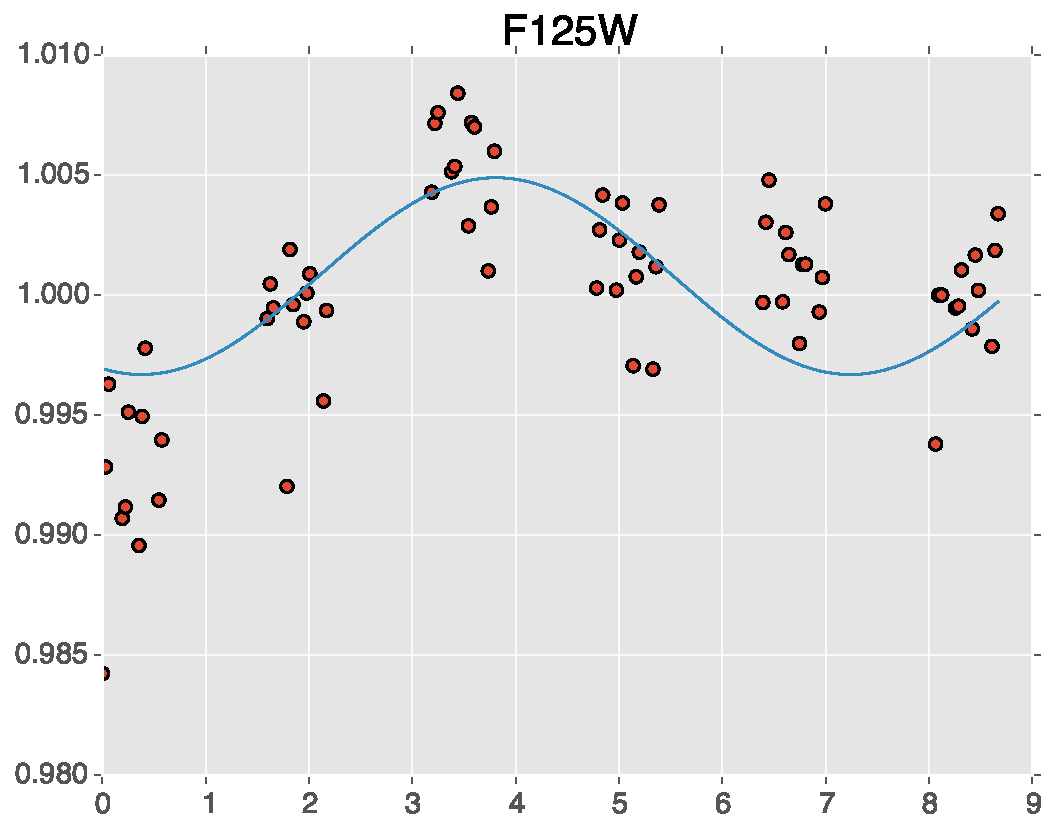
\includegraphics[width=0.8\textwidth]{sineCurveFit_primary}
  \caption{sine wave fitting for 2M1207A.}
  \label{fig:3}
\end{figure}

\embed{
(c) I assume the 10.9 hour fit came from a least-squares analysis --
not quite a full observing/sampling period.  "By eye" it certainly
loooks good, but might be interesting to also do a simple periodogram
analysis, just to see if this might be an alias?}

I thought about this idea before. However, 10.9 hour is longer than the
observation baseline and we if that were the case, we did not have a
periodical signal. I was wondering whether the periodogram would work
for data that does not cover a whole period.

\end{document}
%%% Local Variables:
%%% mode: latex
%%% TeX-master: t
%%% End:
